\begin{frame}
	\frametitle{Heuristic DPLL algorithms}

   	\onslide<1->{
   	\tikzstyle{vertex2} = [opacity = 0]
   	\tikzstyle{vertex3} = [opacity = 0]
    \tikzstyle{vertex4} = [opacity = 0]
   	\tikzstyle{vertex5} = [opacity = 0]
    \tikzstyle{vertex9} = [opacity = 0]
    \tikzstyle{vertex11} = [opacity = 0]
}
\only<2->{\tikzstyle{vertex2} = [opacity = 1]}
\only<3->{\tikzstyle{vertex3} = [opacity = 1]}
\only<4->{\tikzstyle{vertex4} = [opacity = 1]}
\only<5->{
  	\tikzstyle{vertex5} = [opacity = 1]
    \tikzstyle{vertex9} = [opacity = 1]
}

\tikzstyle{end} = [circle, minimum size = 0.6cm, draw, inner sep = 0.1pt]
            
\tikzstyle{level 1} = [level distance = 1.5cm, sibling distance = 5cm]
\tikzstyle{level 2} = [sibling distance = 2cm]
    
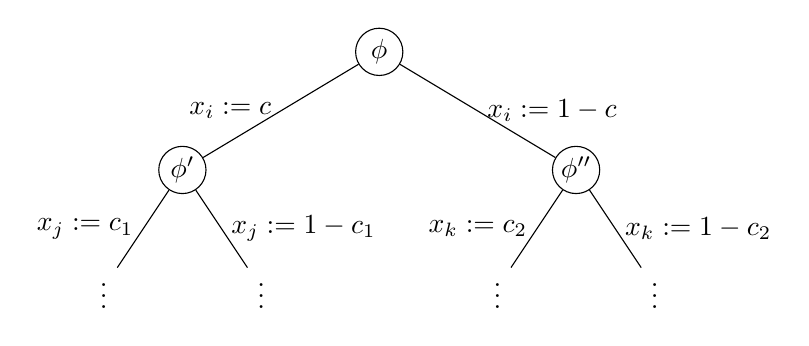
\begin{tikzpicture}[label distance = 8mm]
	\node [end] (z){$\phi$}
       	child [vertex2] {node [end] (b) {$\phi'$}
			child [vertex3]{
	           	node {$\vdots$}
                edge from parent
	  	        node[left] {$x_{j} := c_1$}
            }
		    child [vertex4]{
               	node {$\vdots$}
                edge from parent
	   	        node[right] {$x_{j} := 1 - c_1$}
            }
           	edge from parent
            node[left] {$x_{i} := c$}
        }
        child [vertex5] {node [end] (c) {$\phi''$}
           	child [vertex9]{
               	node {$\vdots$}
                edge from parent
	            node[left] {$x_{k} := c_2$}
            }
		    child [vertex9]{
               	node {$\vdots$}
                edge from parent
	            node[right] {$x_{k} := 1 - c_2$}
            }
            edge from parent
	   	    node[right] {$x_{i} := 1 - c$}
        };
\end{tikzpicture}

    
	\pause
    \pause
    \pause
    \pause
    \pause
    \begin{itemize}
        \item Heuristic $\mathbf{A}$ chooses a variable for splitting.
    	\pause
	    \item Heuristic $\mathbf{B}$ chooses first value.
    \end{itemize}

    \pause
    It's allowed algogithm to have an error.

    \pause
    \pause
    \begin{itemize}
	    \item Heuristic $\mathbf{C}$ cuts branches.
    \end{itemize}
\end{frame}

\begin{frame}
    \frametitle{Lower bounds for DPLL algorithms without cut heuristic}

    \pause
	\begin{itemize}
		\item Unsatisfiable formulas
		\begin{itemize}
            \item{} Exponential lower bounds for resolution refutations
				of unsatisfiable formulas translate to backtracking
                algorithms.
			\item{} [Tseitin, 1968] ... [Pudlak, Implagliazzo, 2000].
		\end{itemize}
        \pause
		\item Satisfiable formulas
		\begin{itemize}
			\item If $\bf P = NP$ then there are no superpolynomial
		        lower bounds for backtracking algorithms since
                heuristic $\mathbf{B}$ may choose correct value.
            \pause
			\item Inverting of functions corresponds to satisfiable
		        formulas.
            \pause
            \item{} [Nikolenko~2002], [Achilioptas, Beame, Molloy~2003-2004]
				exponential lower bound for specific backtracking
                algorithms.
            \item{} [Alekhnovich, Hirsch, Itsykson~2005] Exponential lower bound 
				for myopic and drunken algorithms.
            \pause
            \item{}  Exponential lower bound 
		for inversion of Goldreich's function by myopic [J. Cook et al.~2009] 
		and drunken [Itsykson~2010] algorithms.
%            \item{}  Exponential lower bound 
%				for inversion of Goldreich's function by drunken algorithms.
		\end{itemize}
	\end{itemize}
\end{frame}


\begin{frame}
	\frametitle{Myopic heuristics}
    \pause

    \begin{definition}
        Myopic heuristic:
        \pause
        \begin{itemize}
	        \item sees structure of the formula;
        	\pause
        	\item doesn't see negation signs;
        	\item<6-> requests negations in $K = n^{1 - \epsilon}$ clauses.
        \end{itemize}
    \end{definition}

    \pause
    $\begin{array}{l}
        (x_1 \vee x_3 \vee x_5) \\
        \alert<7->{(x_2 \vee x_3)} \\
        (x_2 \vee x_4 \vee x_5) \\
        \alert<7->{(x_1 \vee x_4 \vee x_6)} \\
    \end{array}
    \pause
    \pause
    \pause
    \Rightarrow
    \begin{array}{l}
        (x_1 \vee x_3 \vee x_5) \\
        (x_2 \vee \alert{\neg} x_3) \\
        (x_2 \vee x_4 \vee x_5) \\
        (x_1 \vee \alert{\neg} x_4 \vee x_6) \\
    \end{array}$
    
\end{frame}

\begin{frame}
    \frametitle{Myopic algorithms}

    \pause

    \begin{definition}
		Myopic algorithm:
        \begin{itemize}
            \pause
	        \item $\mathbf{A}, \mathbf{C}$ are myopic, polynomial, determinate heuristic.
            \pause
        	\item $\mathbf{B}$ can be any.
        \end{itemize}
	\end{definition}

    \pause
    If $\mathbf{C} = 1$, then there exist some bounds: 

    \pause
    \begin{columns}
        \begin{column}{5cm}
            
            polynomial time (upper bound):
        \end{column}
        \begin{column}{5cm}
            
            exponential time (lower bound):
        \end{column}
    \end{columns}

    \pause
    \begin{columns}
        \begin{column}{5cm}
            \begin{itemize}
		 		\item $2$-CNF formulas;
			    \pause
    			\item horn formulas.
            \end{itemize}
        \end{column}
        \begin{column}{5cm}
            \begin{itemize}
	            \pause
    	        \item some classes of unsatifiable formulas;
        		\pause
            	\item formulas, which encode system of linear
		            equatitions.
            \end{itemize}
        \end{column}
    \end{columns}
\end{frame}

\begin{frame}
	\frametitle{Main theorem}
	\pause
	\begin{theorem}
        Для любой детерминированной полиномиальной эвристики $\mathbf{A}$
        существует семейство $(\Phi_n, \mathcal{D}_n)$ и $\delta \ne
        \delta(n)$ такие, что:
        \pause
		\begin{itemize}
            \item $\Phi_n$~--- невыполнимая формула, которую можно
		        построить полиномиальным алгоритмом.
            \pause
            \item $\mathcal{D}_n$~--- распределение на выполнимых
		        формулах, которое моделируется полиномиальным алгоритмом.
            \pause
			\item $\forall \mathbf{B}, \mathbf{C}$,
				$\Pr\limits_{x \gets \mathcal{D}_n}[\mathcal{A}(x)
                \ne 0] > 1 - \epsilon \Rightarrow
                t(\mathcal{A}(\Phi_n)) \ge 2^{\Omega(min(n^\delta,
                \frac{n}{K}))}$, где $\mathcal{A}$~--- близорукий
			    алгоритм $\mathcal{A}(\mathbf{A}, \mathbf{B},\mathbf{C})$.
		\end{itemize}
	\end{theorem}
\end{frame}

\begin{frame}
    \frametitle{Distribution for all algorithms}

    \begin{theorem}
        Существует семейство $(\Phi_n, \mathcal{D}_n)$ и $\delta \ne
        \delta(n)$ такие, что:
        \pause
        \begin{itemize}
	        \item $\Phi_n$~--- невыполнимая формула, которую можно
		        построить полиномиальным алгоритмом.
            \pause
            \item $\mathcal{D}_n$~--- распределение на выполнимых
		        формулах, которое моделируется полиномиальным алгоритмом.
            \pause
            \item $\forall \mathbf{A}, \mathbf{B}, \mathbf{C}$ 
		        если $\exists n_0, \epsilon$ такие, что:
				$\forall n > n_0, ~~ \Pr\limits_{x \gets \mathcal{D}_n}[\mathcal{A}(x)
                \ne 0] > 1 - \epsilon$, то
                $\forall n > n_0, ~~ t(\mathcal{A}(\Phi_n)) \ge 2^{\Omega(min(n^\delta,
                \frac{n}{K}))}$, где $\mathcal{A}$~--- близорукий
			    алгоритм $\mathcal{A}(\mathbf{A}, \mathbf{B},\mathbf{C})$.
        \end{itemize}
    \end{theorem}
\end{frame}

\begin{frame}
	\frametitle{Goldreich's function}
	$f:\{0, 1\}^n \rightarrow \{0, 1\}^n$

    \pause

    \begin{columns}
    	\begin{column}{5.5cm}
            \tikzstyle{end} = [circle, minimum width = 4pt, fill, inner sep = 1pt,
	opacity = 1]
\tikzstyle{start} = [circle, inner sep = 1pt, opacity = 1]
            
\tikzstyle{level 1} = [level distance = 0.1cm, sibling distance = 0.4cm]
\tikzstyle{level 2} = [level distance = 0.45cm]
\tikzstyle{level 3} = [level distance = 1cm]
\tikzstyle{level 4} = [level distance = 0.4cm]

\begin{tikzpicture}[grow = right]
    \node [start]{}
    	child {
        	node [start] (xn) {$x_{n}$}
            	child [end]{
                	node [end] (xvn){}
                    	child [end]{
                        	node [end] (yvn){}
                            	child [start]{
                                	node [start] (yn){}
                                    edge from parent [opacity = 1]
                                }
                            edge from parent [opacity = 0]
                        }
                    edge from parent [opacity = 1]
                }
            edge from parent [opacity = 0]
        }
    	child foreach \i in {3, 2, 1}{
	    	node [start] {}
            	child [start]{
                	node [start] {.}
                    	child [start]{
                        	node [start] {.}
                            edge from parent [opacity = 0]
                        }
                    edge from parent [opacity = 0]
                }
            edge from parent [opacity = 0]
        }
    	child foreach \i in {3, 2, 1}{
	    	node [start] (x\i) {$x_{\i}$}
            	child [end]{
                	node [end] (xv\i){}
                    	child [end]{
                        	node [end] (yv\i){}
                            	child [start]{
                                	node [start] (y\i){}
                                    edge from parent [opacity = 1]
                                }
                            edge from parent [opacity = 0]
                        }
                    edge from parent [opacity = 1]
                }
            edge from parent [opacity = 0]
        };

    \path [draw = red, opacity = 1](xv2) -- (yv2);
    \path [draw = red, opacity = 1](xv3) -- (yv2);
    \path [draw = red, opacity = 1](xvn) -- (yv2);
    \node at (xvn.south) [below = 0.05cm] {$X$};
    \node at (yvn.south) [below = 0.05cm] {$Y$};
    \node <.(2)-> at (y2.east) [right = 0.1cm] {$x_{2} \oplus x_{3}
	    \oplus \dots \oplus x_{n}$};
\end{tikzpicture}

        \end{column}

        \pause
        \pause
        \begin{column}{5.5cm}
            \begin{itemize}
	            \item $f$ is a linear;
            	\pause
                \item $\forall y \in Y ~~ deg(y) \le d$
            	\pause
            	\item $d$ is a constant.
            \end{itemize}
        \end{column}
	\end{columns}
    
	\pause
    \begin{itemize}
	    \item $f_{G, P}(x) = b \Leftrightarrow \Phi(x)$;
    	\pause
	    \item $\Phi(x)$ contains no more than $2^dn$ clauses;
    	\pause
    	\item It's easy to create $\Phi(x)$.
    \end{itemize}
\end{frame}

\begin{frame}
    \frametitle{Dependencies graph}

    Bipartite grapth $(X, Y, E)$
    \pause
    \begin{itemize}
	    \item Full rank of adjacency matrix (over $\mathbb{F}_2$).
    	\pause
        \item $\forall z \in X \cup Y, ~~ deg(z) \le d$, ~~ $d$ is a constant.
    	\pause
        \item Expansion property.
    \end{itemize}

    \pause

    \begin{columns}
        \begin{column}{5cm}
            \tikzstyle{start} = [circle, inner sep = 0pt, opacity = 1]
\tikzstyle{end} = [circle, minimum width = 4pt, fill, inner sep = 1pt,
	opacity = 1]

\onslide<1->{
	\tikzstyle{endY} = [color = black, circle, minimum width = 4pt,
	    fill, inner sep = 1pt, opacity = 1]
	\tikzstyle{endG} = [color = black, circle, minimum width = 4pt,
	    fill, inner sep = 1pt, opacity = 1]
    \tikzstyle{edge} = [draw = black, opacity = 0]
}
\only<6->{
  	\tikzstyle{endY} = [color = red, circle, minimum width = 4pt,
	    fill, inner sep = 1pt, opacity = 1]
    \tikzstyle{edge} = [draw = black, opacity = 1]
}

\only<7->{
  	\tikzstyle{endG} = [color = green, circle, minimum width = 4pt,
	    fill, inner sep = 1pt, opacity = 1]
}
            
\tikzstyle{level 1} = [level distance = 0.1cm, sibling distance = 0.4cm]
\tikzstyle{level 2} = [level distance = 1.5cm]
\tikzstyle{level 3} = [level distance = 1cm]

\begin{tikzpicture}[grow = right]
    \node [start]{}
    	child foreach \i in {10, 9}{
            node [end] (x\i) {}
               	child [end]{
	             	node [end] (y\i){}
    	            edge from parent [opacity = 0]
        	    }
            edge from parent [opacity = 0]
        }
        child foreach \i in {8, ..., 7}{
            node [end] (x\i) {}
               	child [endY]{
	             	node [endY] (y\i){}
    	            edge from parent [opacity = 0]
        	    }
            edge from parent [opacity = 0]
        }
        child foreach \i in {6, ..., 2}{
            node [endG] (x\i) {}
               	child [end]{
	             	node [end] (y\i){}
    	            edge from parent [opacity = 0]
        	    }
            edge from parent [opacity = 0]
        }
        child {
        	node [end] (x1) {}
           		child [end]{
	          		node [end] (y1){}
	    	        edge from parent [opacity = 0]
                }
    	   	edge from parent [opacity = 0]
        };

	\path [edge](y8) -- (x6);
    \path [edge](y8) -- (x4);
    \path [edge](y8) -- (x2);
    \path [edge](y7) -- (x3);
    \path [edge](y7) -- (x5);
    \path [edge](y7) -- (x6);

    \node at (x10.south) [below = 0.05cm] {$X$};
    \node at (y10.south) [below = 0.05cm] {$Y$};

    \path [opacity = 0](y7) -- (y8) node [start, midway] (mid){};
    \node <.(2)-> at (mid.east) [right = 0.05cm] {$J$};
    \node <.(3)-> at (x4.west) [left = 0.05cm] {$\Gamma(J)$};
\end{tikzpicture}
        \end{column}

        \pause
        \pause
        \pause
        \begin{column}{5cm}
            \begin{itemize}
                \item $\forall y \in Y ~~ deg(y) \le d$
            	\pause
	            \item $\forall J \subset Y, ~
            		|J| < r \Rightarrow \Gamma(J) \ge \frac{3}{4}d|J|$
            \end{itemize}
		\end{column}
    \end{columns}

\end{frame}

\begin{frame}
	\frametitle{Idea of the proof}

    \pause
    Носитель распределения на выполнимых формулах состоит из
    модификаций невыполнимой формулы.
	\pause
    \begin{itemize}
        \item $\Phi_n$ кодирует задачу обращения функции Голдрейха.
    	\pause
    	\item $\Phi_n \mapsto \mathcal{D}_n, ~ |supp(\mathcal{D}_n)| =
		    2^{min(n^\delta, \Omega(\frac{n}{K}))}$ так, чтобы корректная
		    работа на конкретной выполнимой формуле означала
            ``увеличение времени работы на 1''.
	\end{itemize}

    \pause
    Построение единого распределения для всех близоруких DPLL
    алгоритмов:
    
    \pause
    \begin{itemize}
        \item комбинирование распределений из основной теоремы.
    \end{itemize}
\end{frame}

\begin{frame}
    \frametitle{Результаты}

    \pause
    \begin{enumerate}
	    \item Теорема о ``компромиссе''. Если близорукий алгоритм работает
		    корректно на построенном распределении, то он работает долго, на
		    построенной формуле.
        \pause
        \item Построение единого распределения для всех близоруких алгоритмов.
        \pause
        \item Конструкция экспандеров с полным рангом и ограниченной
		    степенью всех вершин.
    \end{enumerate}
\end{frame}